\chapter[Referencial Teórico]{Referencial Teórico}
\label{cap:referencial}

Este capítulo irá tratar dos conceitos teóricos necessários para a realização deste 
Trabalho de Conclusão de Curso. Este trabalho tem como objetivo gerar contribuições 
para as áreas de \textit{Design} de \textit{Software} e Técnicas de Programação em Desenvolvimento \textit{Mobile}.

Primeiramente, são abordados os temas de \textit{Design} de \textit{Software} (\ref{sectionDesign}) e Técnicas de Programação (\ref{sectionTecnicas}), 
que são áreas de interesse do trabalho por englobarem o DDD (\textit{Domain Driven Design}) e o TDD 
(\textit{Test Driven Development}). Após isso, o capítulo detalha o \textit{Story Slicing} (\ref{sectionStorySlicing}), tema  
importante para a divisão das tarefas que serão implementadas na parte prática do trabalho.
Depois, são passados pelos temas de Desenvolvimento \textit{Mobile} (\ref{sectionMobile}), 
Engenharia Reversa (\ref{sectionEngReversa}) e Reengenharia (\ref{sectionReengenharia}), por serem temas pertinentes à proposta do trabalho de 
contribuir com uma aplicação móvel. Por fim, são feitas Considerações Finais (\ref{sectionConsideracoes}) sobre o capítulo, 
repassando os principais pontos abordados durante o mesmo.

\section{\textit{Design} de \textit{Software} }
\label{sectionDesign}

\subsection{Definição}

Segundo \citeauthoronline{robert2019clean} (\citeyear{robert2019clean}), o \textit{Design} de \textit{Software} e 
a Arquitetura de \textit{Software} não possuem nenhuma diferença e, por definição, são o detalhamento com um conjunto 
de princípios, normas e técnicas utilizadas no desenvolvimento de um sistema, sendo um processo fundamental, 
seja ele uma solução web ou um aplicativo. Sem ele, o \textit{software} acaba ficando sucetível a diversos 
problemas futuros tanto em relação a manutenção, quanto a evolução.

O \textit{design} de \textit{software} é, também, um processo que envolve revisões contínuas. 
Visto que, à medida que o \textit{software} é desenvolvido e testado, podem surgir necessidades 
de ajustes no \textit{design} inicial. Assim como uma ponte bem projetada deve ser capaz de 
suportar cargas e resistir ao tempo, um \textit{design} de \textit{software} eficaz é essencial 
para criar sistemas eficientes de forma confiável e escalável.

\subsection{Princípios do \textit{Design}}

Construir um sistema pode ser uma tarefa desafiadora, tendo em vista que não existe uma arquitetura 
pré definida para atender todo e qualquer tipo de solução. Cabe ao arquiteto de software analisar 
e decidir qual caminho seguir para um \textit{design} de qualidade.

O desenvolvimento de \textit{software} é uma área que está em constante evolução, e a qualidade do 
código desempenha um papel vital no seu sucesso. Segundo \citeauthoronline{robert2019clean} (\citeyear{robert2019clean}), a única maneira de 
otimizar esse desenvolvimento é escrever um código limpo. Isso ressalta a importância dos princípios de \textit{design} de 
\textit{software} na criação de código limpo e de alta qualidade. Com isso, alguns princípios acabaram surgindo 
no contexto do \textit{design} de \textit{software}, estes são conhecidos como SOLID \cite{robert2019clean}.

O acrônimo SOLID simboliza cinco princípios de \textit{design} de \textit{software} que foram criados 
para desenvolver sistemas de \textit{software} de uma maneira mais compreensível, concisa, flexível e 
de fácil manutenção, são eles:

\begin{itemize}

	\item SRP - Princípio da Responsabilidade Única (\textit{Single Responsibility Principle}): Estabelece 
    que uma classe ou módulo deve ter apenas uma razão para mudar. Em outras palavras, uma classe deve ter 
    uma única responsabilidade bem definida. Isso promove o design de componentes de software mais coesos 
    e facilita a manutenção, uma vez que as alterações afetam apenas uma área específica;
	\item OCP - Princípio do Aberto/Fechado (\textit{Open/Closed Principle}): Afirma que um componente de 
    \textit{software} deve estar aberto para extensão, mas fechado para modificação. Isso significa que novas 
    funcionalidades podem ser adicionadas sem alterar o código existente, promovendo sistemas flexíveis 
    e facilmente expansíveis;
	\item LSP - Princípio da Substituição de Liskov (\textit{Liskov Substitution Principle}): Enfatiza que 
    as subclasses devem ser substituíveis por suas classes base sem afetar o comportamento do programa. 
    Isso garante que a herança seja utilizada de forma coerente e que as classes derivadas mantenham o 
    mesmo contrato das classes base;
	\item ISP - Princípio da Interface Segregada (\textit{Interface Segregation Principle}): Recomenda que 
    as interfaces sejam específicas para as necessidades dos clientes, evitando interfaces monolíticas. 
    Isso ajuda a evitar a implementação de métodos desnecessários e promove a coesão nas classes que 
    implementam essas interfaces, e
	\item DIP - Princípio da Inversão de Dependência (\textit{Dependency Inversion Principle}): Sugere que 
    os módulos de alto nível não devem depender diretamente dos módulos de baixo nível, mas sim de abstrações. 
    Isso promove a flexibilidade e a reutilização de componentes, permitindo que diferentes implementações 
    sejam facilmente substituídas.
    
\end{itemize}

\section{Técnicas de Programação}
\label{sectionTecnicas}

\subsection{Visão Geral}

A sociedade atual está cada vez mais orientada pela tecnologia. Nesse cenário, a tecnologia possui um papel 
extremamente importante na criação de soluções de \textit{software}, bem como aplicativos, sistemas e plataformas 
que impulsionam a vida digital e o mercado. Porém, desenvolver um \textit{software} eficaz e confiável 
é um grande desafio. Isso requer conhecimento técnico, bom planejamento e aplicação de métodos adequados para atingir 
os principais objetivos relacionados à qualidade de \textit{software}.

As técnicas de programação são abordagens utilizadas no desenvolvimento de \textit{software} para solucionar 
problemas, organizar o código e criar sistemas que atendam as necessidades do mercado. Elas visam aprimorar 
a qualidade, manutenibilidade e a eficiência do código. Dessa forma tanto o desenvolvimento quanto as equipes 
se tornam mais eficientes.

Existem diversas técnicas de programação dentro da Engenharia de \textit{Software}, cada uma com sua particularidade. 
A compreensão e a aplicação de forma correta dessas técnicas é de extrema importância em um cenário onde a tecnologia 
está em constante evolução e demanda cada dia mais por soluções de \textit{software} no mercado em diversas áreas.

\subsection{TDD (\textit{Test Driven Development})}

Uma técnica de programação comum na Engenharia de \textit{Software} é o TDD (\textit{Test Driven Development}), 
que é uma abordagem que busca, principalmente, otimizar o desenvolvimento e aumentar a confiabilidade do código. Essa abordagem 
visa a escrita dos testes unitários antes do desenvolvimento de qualquer linha de código funcional, sendo um processo dividido 
em três etapas:

\begin{itemize}

	\item Escrita do teste (\textit{Red})- Nessa etapa, o foco é escrever os testes unitários relacionados à funcionalidade, 
    \textit{feature} ou \textit{user story} a ser implementada, sempre visando cobrir o maior número de casos possíveis. porém, 
    como essa funcionalidade ainda não foi escrita, o teste resulta em falha, por isso o termo \textit{Red} (Vermelho na tradução);
	\item Escrita do código (\textit{Green})- Nessa etapa, o foco é a escrita da funcionalidade em si para que os testes sejam 
    atendidos e resultem em sucesso, fazendo com que o \textit{Red} se torne \textit{Green} conforme o esperado, e
	\item Refatoração do código (\textit{Refactor})- Nessa etapa, após o código e seus respectivos teste funcionais, o foco é o 
    aprimoramento do código visando uma melhor estrutura e organização. Dessa forma é garantida sua maior eficácia, confiabilidade e 
    manutenibilidade.
    
\end{itemize}

Tais etapas podem ser visualizadas na Figura \ref{fig02} \cite{DevCommunity}.

\begin{figure}[h]
	\centering
	\caption{Ciclo do \textit{Test-Driven Development}}
	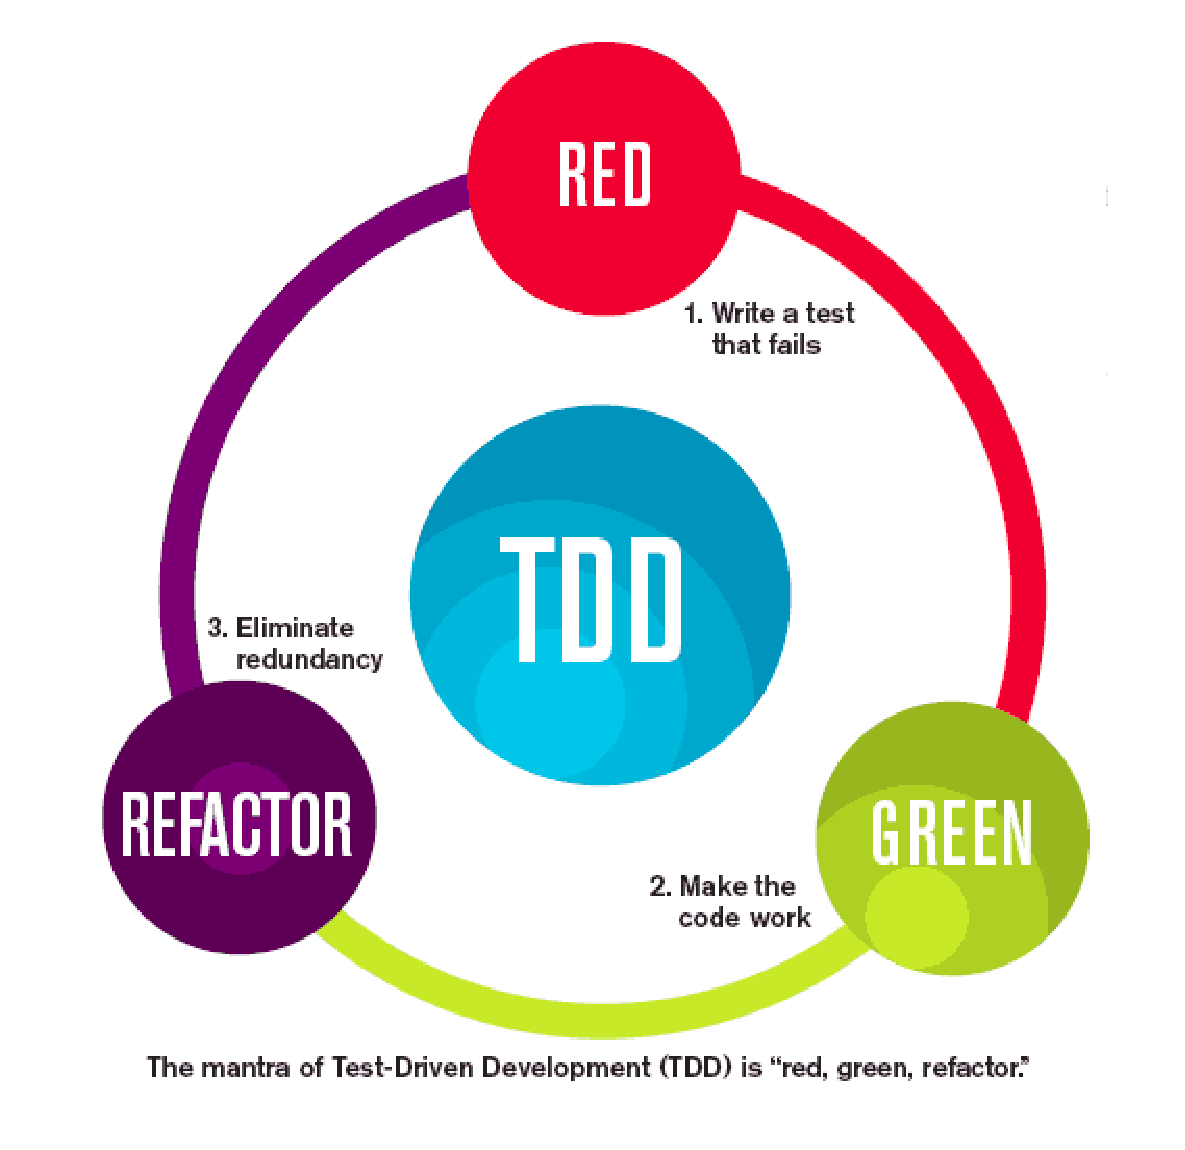
\includegraphics[keepaspectratio=true,scale=0.4]{figuras/fig02.eps}
	\parbox{\linewidth}{\centering FONTE: \cite{DevCommunity}}
	\label{fig02}
\end{figure}

\section{\textit{Story Slicing}}
\label{sectionStorySlicing}

O \textit{Story Slicing}, ou \textit{Story Splitting}, é essencialmente a divisão das histórias de 
usuário em níveis de granularidade menores, criando subtarefas programáveis. Com isso, é 
possível gerar valor para os usuários com rapidez, possuindo adequada familiaridade com o ciclo do 
desenvolvimento ágil. Além disso, a técnica de desenvolvimento do TDD pode se beneficiar desta metodologia, 
os níveis de granularidade menores gerados como blocos de funcionalidades que serão implementadas
em suas etapas \cite{beck2022test}. Existem duas abordagens para o \textit{Story Slicing}, sendo elas 
o fatiamento horizontal e vertical.

O fatiamento vertical é quando as histórias de usuário são subdivididas verticalmente,
de maneira com que os blocos menores ainda resultem em uma funcionalidade
que além de ser funcional, possa ser demonstrada, sendo assim útil para os usuários. De
maneira geral, pode-se pensar que essa abordagem utiliza de várias camadas técnicas
para a implementação de uma fatia. Um exemplo dessa abordagem é a definição de uma
subtarefa que, para ser concluída, necessita de implementações na camada gráfica, no
banco de dados e nas configurações da aplicação, sendo essas diferentes camadas técnicas
do \textit{software} \cite{StorySlicing}.

\begin{figure}[h]
	\centering
	\caption{\textit{Story Slicing} Vertical}
	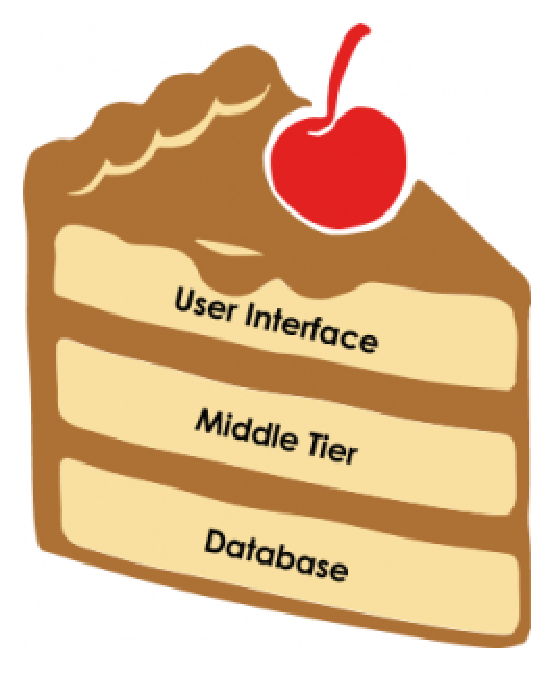
\includegraphics[keepaspectratio=true,scale=0.6]{figuras/storyslicing_vertical.eps}
	\parbox{\linewidth}{\centering FONTE: \cite{StorySlicing}}
	\label{fig_storyslicing}
\end{figure}

Já no fatiamento horizontal, pensa-se na divisão baseada nas camadas técnicas
existentes na aplicação, podendo assim combinar com as habilidades específicas do time
de desenvolvimento. Nesta abordagem, cada subtarefa irá interagir apenas com a camada
técnica definida para a mesma. Um exemplo de utilização desta abordagem é a definição
de subtarefas de uma história de usuário em que uma fatia implementa apenas a parte do
banco de dados; enquanto outra implementa a parte gráfica da mesma história de usuário
original. Com a utilização desta funcionalidade, as subtarefas, na maioria das vezes, só irão
agregar valor para os usuários quando elas integrarem entre si \cite{StorySlicing}.

Visto as características das abordagens vertical e horizontal, pode-se perceber que
a primeira é mais interessante quando o objetivo é entregar pequenos blocos de funcionalidade
que agreguem valor aos usuários, e que também interajam com diversas camadas
técnicas do projeto. Enquanto a segunda, torna-se mais interessante quando o time de desenvolvimento
possui habilidades mais especializadas, e que cada funcionalidade é pensada
para interagir apenas com uma camada técnica do \textit{software}.

\section{Desenvolvimento \textit{Mobile}}
\label{sectionMobile}

O uso exponencial de dispositivos móveis nos últimos anos tem sido notável no cotidiano da população em todas as faixas etárias, 
abrangendo desde a comunicação até tarefas mais complexas, conforme apontado por dados da \cite{FGV}. No Brasil, o registro de, 
aproximadamente, 464 milhões de dispositivos digitais, incluindo computadores, \textit{notebooks} e \textit{tablets}, destaca-se 
especialmente pelos 249 milhões de \textit{smartphones} em uso, o que equivale a mais de um dispositivo móvel por habitante, conforme dados 
também fornecidos pela \cite{FGV}. Essa proliferação de dispositivos móveis tem gerado diversas consequências, como mencionado por 
\cite{coutinho2014era}.

Paralelamente, observa-se um aumento significativo nos investimentos em equipes de Tecnologia da Informação nas empresas, com um 
custo anual médio de aproximadamente 52 mil reais por usuário, conforme evidenciado na Figura \ref{fig_dev_mobile}.

\begin{figure}[h]
	\centering
	\caption{Média de Gastos de Investimentos em TI}
	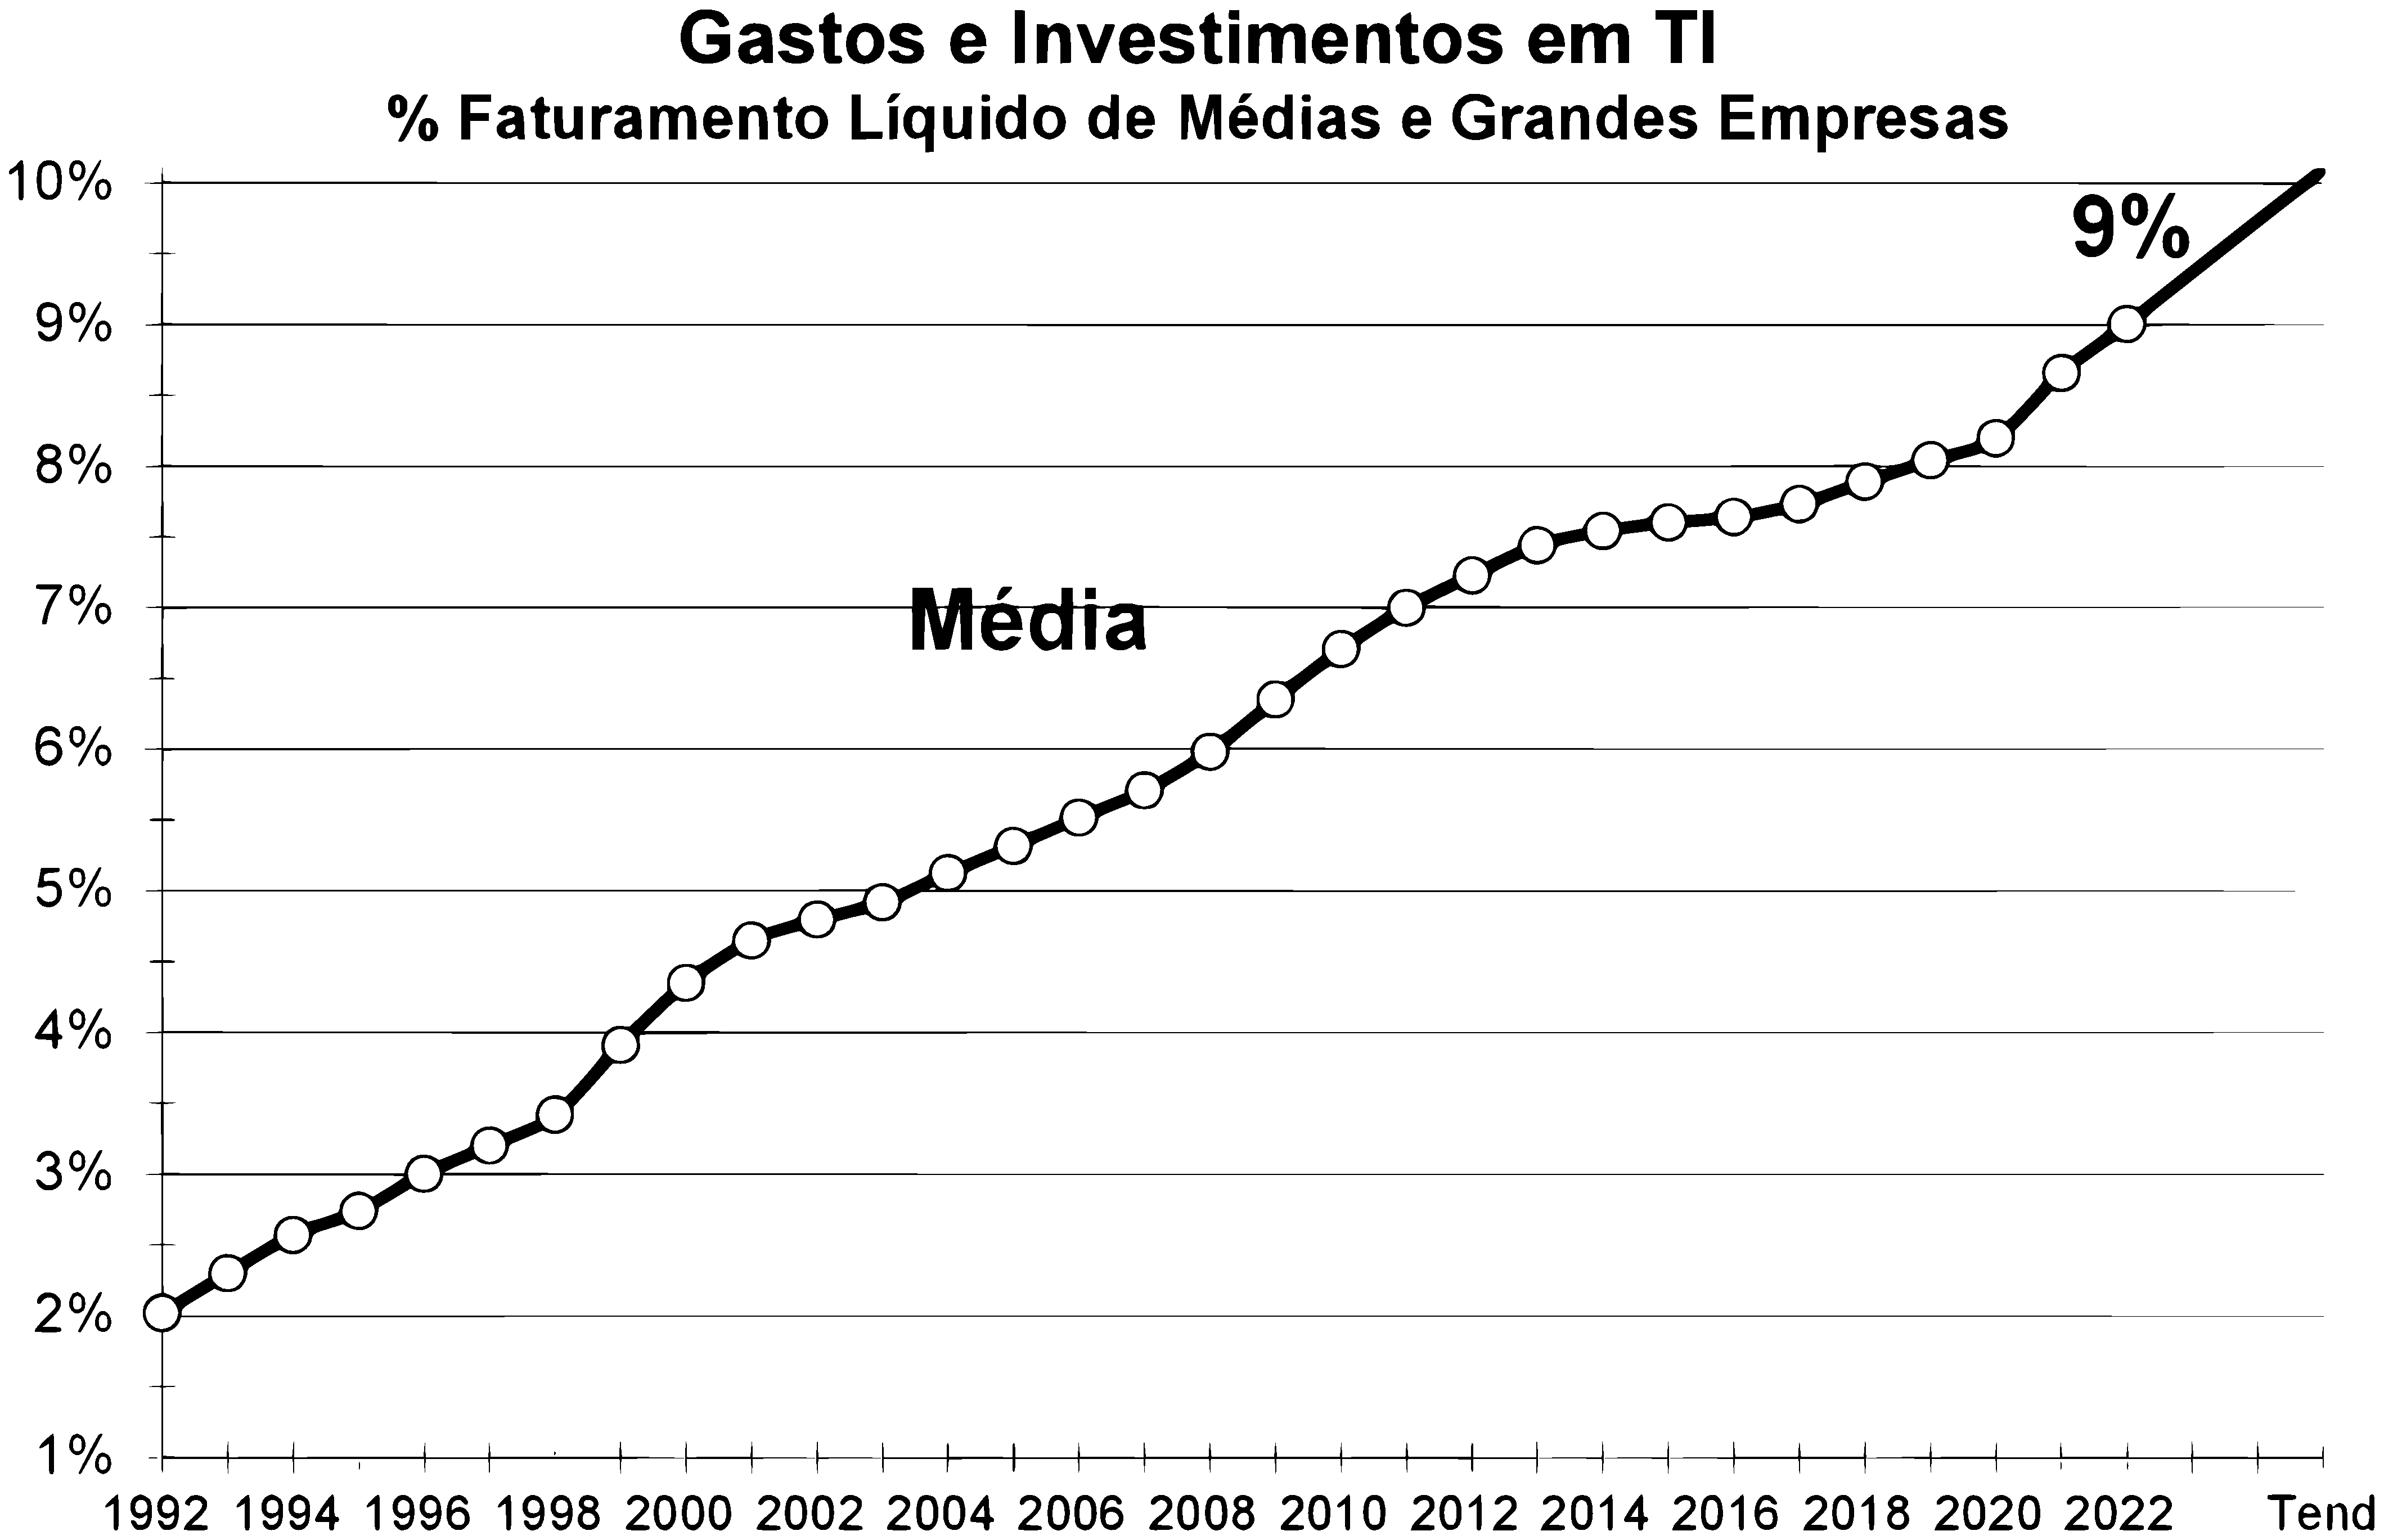
\includegraphics[keepaspectratio=true,scale=0.2]{figuras/fig_dev_mobile.eps}
    \parbox{\linewidth}{\centering FONTE: \cite{FGV}}
	\label{fig_dev_mobile}
\end{figure}

Diante desse cenário e do considerável avanço das tecnologias, percebe-se uma clara tendência de crescimento de soluções direcionadas 
ao público de dispositivos móveis. Destacam-se aplicativos voltados para serviços de entrega, comunicação por meio de bate-papo e 
reuniões \textit{online}. Nesse contexto, o conceito de \textit{mobile first} ganha destaque, indicando que o desenvolvimento dessas 
soluções tem como prioridade atender, majoritariamente, aos dispositivos móveis.

Nos últimos anos, o desenvolvimento \textit{mobile} tem testemunhado uma evolução significativa. O destaque vai para o crescimento do desenvolvimento 
multiplataforma, impulsionado por \textit{frameworks} como React Native e Flutter \cite{freitas2022flutter}. Essas ferramentas permitem a criação eficiente de 
aplicativos a partir de um único código-base, agilizando o processo de desenvolvimento.

Garantir a qualidade em desenvolvimento \textit{mobile} é crucial, sendo possível com testes de unidade e integração \cite{santos2015definiccao}, fundamental para 
assegurar a estabilidade dos componentes do aplicativo. Além disso, existem os testes de aceitação do usuário (UI/UX), que se concentram na 
experiência do usuário final \cite{melo2023ux}. Por fim, o monitoramento contínuo após o lançamento do aplicativo permite uma resposta às falhas, 
contribuindo para melhorias sucessivas na qualidade do \textit{software}.

\newpage
\section{Engenharia Reversa}
\label{sectionEngReversa}

\subsection{Definição}

De acordo com \citeauthoronline{eilam2011reversing} (\citeyear{eilam2011reversing}), a engenharia reversa é o 
processo de extrair conhecimento a partir de algo feito 
pelo ser humano. Este conceito existe desde antes dos computadores e da tecnologia moderna, e se 
assemelha muito à pesquisa científica clássica, tendo como diferença o objeto de estudo, que é algo 
produzido pelo homem, e não um fenômeno natural.

A engenharia reversa, tradicionalmente desmonta produtos físicos para descobrir 
os segredos de seu \textit{design}. Um exemplo disso é a prática comum entre as pessoas de, por curiosidade, 
desmontar algum produto eletrônico, como o rádio, para descobrir o funcionamento do mesmo. O conhecimento 
adquirido com esta prática normalmente é utilizado para construir produtos similares ou melhores \cite{eilam2011reversing}.

A evolução da tecnologia vem dificultando cada vez mais esta prática. Os produtos digitais modernos 
estão com peças cada vez menores, o que torna mais difícil a descoberta de funcionamentos a partir 
da desmontagem destes dispositivos. O surgimento dos produtos de \textit{software} também trouxe outra dificuldade 
para esta prática, que por não serem físicos, são impossíveis de serem desmontados. Ainda sim, é possível 
realizar a engenharia reversa em produtos de \textit{software} \cite{eilam2011reversing}.

\subsection{Engenharia Reversa em \textit{Software}}
\label{engenharia-reversa}

Assim como acontece com os produtos físicos na engenharia reversa tradicional, as aplicações de \textit{software} 
também podem ser “desmontadas” a fim de descobrir seu funcionamento e seu \textit{design}. Este processo acontece 
de forma virtual, envolvendo apenas ferramentas computacionais e o raciocínio lógico. \cite{eilam2011reversing}.

A engenharia reversa na Engenharia de \textit{Software} demanda habilidades e entendimento sobre computadores e 
desenvolvimento de \textit{software}. Existem algumas técnicas que compõem este processo, sendo elas: quebra de 
código, resolução de quebra-cabeças, programação e análise lógica. Estas técnicas podem ser aplicadas em 
um arquivo binário de uma aplicação existente, a fim de descobrir suas funcionalidades, ou ainda diretamente 
no código fonte \cite{eilam2011reversing}.

É válido dizer que, na indústria de \textit{software}, a principal motivação para a realização da engenharia reversa 
para descobrir os segredos de um sistema é a de desenvolver aplicações competidoras. Porém, dependendo da 
complexidade da aplicação, torna-se um processo muito custoso, não valendo a pena despender recursos e tempo 
para isso. Nestes casos, desenvolver a aplicação do zero, elicitando os requisitos e funcionalidades necessárias 
se torna um processo mais fácil e mais barato \cite{eilam2011reversing}.

Na área de \textit{hardware}, é comum realizar projetos novos a partir  da engenharia reversa em produtos finalizados. 
Já na área de \textit{software}, a engenharia reversa pode ser utilizada com o intuito de apoiar a manutenção, a evolução 
ou até a substituição de um sistema já implementado. Neste caso, o objetivo principal deixa de ser o de produzir 
uma aplicação competidora, e passa a ser de aprimorar um sistema no qual o código fonte esteja disponível para a 
equipe desenvolvedora \cite{cagnin2005parfait}.

A engenharia reversa, quando utilizada com o objetivo de analisar um sistema em funcionamento, é um processo que 
realiza a abstração em alto nível dos componentes e relacionamentos do projeto. Ela pode ser classificada como 
redocumentação ou recuperação de projeto. Na redocumentação, a engenharia reversa se preocupa em criar ou melhorar a documentação 
sobre o sistema analisado. Já na recuperação de projeto, o objetivo é compreender completamente o sistema, entendendo o que o 
sistema faz, de qual maneira e o porquê de realizar desta forma, para posteriormente, aplicar a reengenharia do sistema \cite{cagnin2005parfait}.

\section{Reengenharia}
\label{sectionReengenharia}

\subsection{Visão Geral}

Segundo \citeauthoronline{chikofsky1990reverse} (\citeyear{chikofsky1990reverse}), existem seis termos que são relacionados à reengenharia de \textit{software}, sendo eles: engenharia 
avante, engenharia reversa, redocumentação, recuperação do projeto, reestruturação e reengenharia. Ao introduzir estes 
termos, os autores tiveram como objetivo racionalizar e padronizar termos que já estavam sendo utilizados na área de 
Engenharia de \textit{Software}. Estes termos são apresentados a seguir:

A engenharia avante consiste na implementação dos requisitos de projeto e modelos lógicos que são abstraídos 
numa fase anterior à de desenvolvimento. A engenharia reversa tem o objetivo de analisar um sistema legado, possuindo 
duas classificações, a de redocumentação e a de recuperação do projeto, como foi explicado na seção \ref{engenharia-reversa}. 
A reestruturação, trata-se de manter a mesma funcionalidade de um sistema, porém, com uma outra implementação, sendo 
um processo também conhecido como refatoração. E por fim, a reengenharia consiste na renovação de um sistema já implementado \cite{chikofsky1990reverse}.

A reengenharia de \textit{software} é o processo de analisar e alterar o sistema, mantendo os requisitos da aplicação original, 
mas aplicando novas abordagens de desenvolvimento. Normalmente, o primeiro passo para se realizar a reengenharia, é a 
realização da engenharia reversa, para conhecer o funcionamento e \textit{design} do produto, para depois realizar a engenharia 
avante ou reestruturação, com o objetivo de re-implementar o sistema de outra forma \cite{cagnin2005parfait}.

Um produto de \textit{software} é algo que passa por constantes evoluções, para satisfazer novas necessidades de seus usuários e 
também para resolver \textit{bugs} \footnote{Segundo o Dicionário Escolar da Língua Portuguesa DICIO, \textit{Bug} significa "Falha 
ou erro num programa informático, dispositivo, \textit{site} etc., que impede o seu funcionamento correto ou causa um mau desempenho" 
\cite{dicio2020online}} existentes no sistema. Estas constantes atividades de manutenção que os desenvolvedores fazem, juntamente com 
a falta de atualizações na documentação do \textit{software}, muitas vezes degradam não só o código fonte, como também o projeto como 
um todo. Estes sistemas degradados, que são difíceis de serem mantidos e evoluídos, mas ainda sim estão em funcionamento, são chamados 
de sistemas legados \cite{cagnin2005parfait}.

\subsection{Reengenharia em Sistema Legado}

No contexto do desenvolvimento de \textit{software}, muitas vezes os desenvolvedores devem lidar com código legado ao invés de desenvolver 
novos códigos. Existem diversos tipos de projetos legados, mas uma característica que normalmente aparece em comum é a dificuldade 
de realizar a manutenção e evolução do código fonte. Esta dificuldade está atrelada a algumas propriedades dos projetos legados, como 
o tempo de existência do projeto, alta quantidade de linhas de código, mudanças dentro do time de desenvolvimento e a má documentação da 
aplicação \cite{birchall2016re}.

De acordo com \citeauthoronline{sneed1995planning} (\citeyear{sneed1995planning}), a reengenharia em projetos legados possui quatro objetivos principais, sendo eles: melhorar a manutenibilidade, 
migrar o sistema, alcançar maior confiabilidade e aumentar a escalabilidade. Existem diversas formas para alcançar estes 
objetivos, como dividir o sistema em módulos menores ou até migrar para uma infraestrutura mais adequada. Ao realizar a reengenharia, 
as funcionalidades originais são preservadas, mas implementadas em uma nova arquitetura, sendo uma grande vantagem desta técnica.

Assim como existem diversos tipos de sistema legado com diversos tipos de problemas e características, também existem diversas formas de 
se conduzir a reengenharia de \textit{software}. Pensando nisso, \citeauthoronline{rosenberg1996software} (\citeyear{rosenberg1996software}) 
propõe quatro tipos de abordagens para se realizar a reengenharia, sendo elas: a “\textit{big bang}”, a incremental, a evolutiva e a híbrida. 
Estas abordagens de reenharia de \textit{software} serão abordadas a seguir.

\begin{itemize}
  
\item A abordagem “\textit{big bang}", assim como o nome sugere, é feita de uma forma que o sistema legado é totalmente trocado por um sistema novo, 
    como pode ser evidenciado na Figura \ref{figReengenharia}(a). A vantagem de se utilizar esta abordagem é a de não precisar ter a compatibilidade entre 
    componentes do sistema anterior com o sistema novo. Já as desvantagens são que esta técnica não é apropriada para grandes sistemas, e 
    também as eventuais alterações no código fonte legado que foram feitas durante o desenvolvimento do novo sistema devem ser implementadas 
    novamente \cite{rosenberg1996software}.

  \item A abordagem incremental é feita de forma gradativa, substituindo aos poucos os componentes do sistema legado por componentes novos, por 
    meio de versões do novo sistema, como pode ser evidenciado na Figura \ref{figReengenharia}(b). As vantagens desta técnica são que a reengenharia em blocos 
    menores é mais veloz e mais fácil de se perceber falhas, e também é possível de se disponibilizar versões para os usuários, conforme os 
    componentes são trocados, podendo ocorrer a validação por meio de testes de aceitação. As desvantagens desta técnica são a de existir a 
    necessidade de um grande controle no ambiente e configuração para os dois sistemas coexistirem, e também por deixar a arquitetura do 
    sistema menos maleável, pois nesta técnica apenas o interior dos componentes são alterados, não havendo uma mudança no \textit{design} da 
    aplicação \cite{rosenberg1996software}.

  \item A abordagem evolutiva, assim como na abordagem incremental, também ocorre de forma gradativa, com a diferença de migrar os componentes 
    baseado em funcionalidades em comum, e não apenas na estrutura, como pode ser visto na Figura \ref{figReengenharia}(c). A grande vantagem desta técnica é 
    a centralização de funcionalidades semelhantes. Já a desvantagem é o de exigir muito esforço em agrupar as funcionalidades em comum que 
    estão espalhadas pelos diversos componentes do sistema legado \cite{rosenberg1996software}.

  \item A abordagem de reengenharia híbrida realiza a migração do sistema legado a partir de abstrações e métodos específicos, 
    como pode ser visto na Figura \ref{figReengenharia}(d). Nesta técnica, o código fonte é utilizado para a criação de um novo projeto para o sistema, no qual 
    são elicitados os requisitos necessários e também é identificado quais funcionalidades do projeto legado estão obsoletas e não precisam 
    constar no novo projeto. E por fim, é realizada a codificação deste novo projeto \cite{rosenberg1996software}.

\end{itemize}

\begin{figure}[h]
	\centering
	\caption{Abordagens de Reengenharia}
	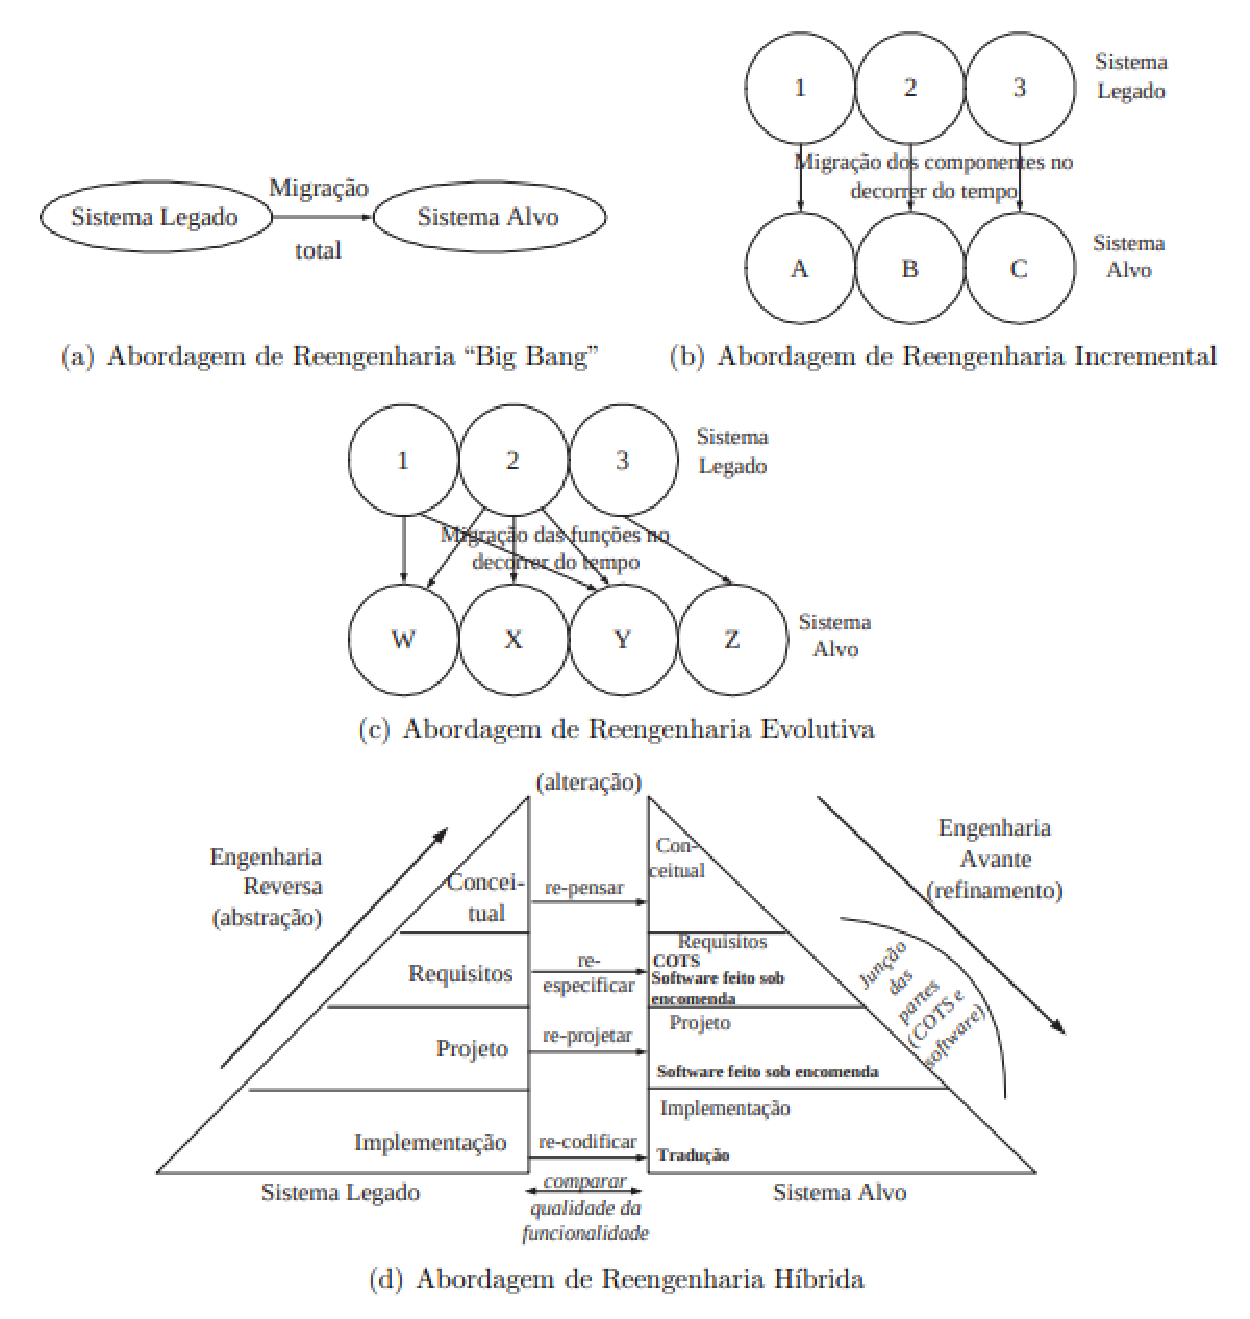
\includegraphics[keepaspectratio=true,scale=0.7]{figuras/abordagens-reengenharia.eps}
    \parbox{\linewidth}{\centering FONTE: \cite{cagnin2005parfait}}
	\label{figReengenharia}
\end{figure}

\section{Considerações Finais do Capítulo}
\label{sectionConsideracoes}

Este capítulo preocupou-se em mostrar uma visão geral sobre os pontos de maior relevância que compõem a fundamentação teórica 
deste trabalho. Primeiramente foram apresentadas conceituações e detalhamentos sobre \textit{Design} de \textit{Software}, para apresentar este 
conceito da Engenharia de \textit{Software} e para mostrar a importância de uma boa escolha de \textit{design} para uma aplicação de qualidade. 
Também é falado sobre o DDD, que é o modelo de \textit{design} escolhido para o novo sistema que será implementado com este trabalho.

Depois, há a abordagem do tema de Técnicas de Programação, na qual é feita uma conceituação e uma explicação da importância da 
utilização de boas técnicas na implementação de um sistema de \textit{software}, para garantir a qualidade e testabilidade do mesmo. 
Além disso, também é apresentado o TDD, que é uma técnica que será utilizada na implementação da aplicação prática deste trabalho.

Outro tópico abordado foi o de Desenvolvimento \textit{Mobile}, que está relacionado ao aplicativo \citeauthoronline{MiaAjuda} (\citeyear{MiaAjuda}), aplicativo este que é o 
alvo das contribuições deste trabalho. Neste tópico são abordadas questões sobre o mercado mobile e também sobre o desenvolvimento 
de aplicativos móveis.

Por fim, são apresentados os conceitos de Engenharia Reversa e Reengenharia, dois tópicos que conversam entre si, visto que o 
primeiro passo para a reengenharia de \textit{software} é a própria engenharia reversa. Nestes tópicos são feitas definições e também 
como estes conceitos são importantes na hora de revitalizar um sistema legado e melhorar sua manutenibilidade.
